\chapter{Production d'une source cohérente d'ondes de matière}
\label{ch:BEC_manip}
%\begin{tikzpicture}[remember picture, overlay]
%\node[anchor=north east,inner sep=0pt] at (current page.north east) {
\includegraphics[scale=1]{Fig/Chapter1/g825.png}};
%\end{tikzpicture}


interaction lumière-atome, BEC, principales étapes de refroidissement. 

Partie précédente = introduction à la physique de cette thèse: propagation d'onde en milieu désordonné. À présent, description de notre source d'ondes de matière: un condensat de Bose-Einstein. Le désordre sera présenté chapitre 4. 

Dans ce chapitre, nous nous attacherons à décrire un condensat de Bose-Einstein et ses principales propriétés, les outils dont nous disposons pour manipuler les atomes, et enfin la manière dont ces outils sont implémentés sur notre expérience.

\section{Condensation de Bose-Einstein}
Commençons par décrire ce qu'est un condensat de Bose-Einstein. Le phénomène de condensation a été prédit par Albert Einstein dans les années 1920 en s'appuyant sur les travaux de Satyendranath Bose traitant des statistiques quantiques pour des particules plus tard appelées \emph{bosons}. Il a cependant fallu attendre les années 1960 et le développement des premiers lasers pour voir émerger les premières techniques de manipulation d'atomes. La mise au point de telles technologies a d'ailleurs valu le prix Nobel à ses principaux architectes Claude Cohen-Tannoudji, Steven Chu et William D. Phillips en 1997. Enfin, le premier condensat de Bose-Einstein gazeux de ${}^{87}$Rb a été obtenu par l'équipe de Eric Cornell et Carl Wieman \citep{anderson1995observation}, rapidement suivi par un condensat de ${}^{23}$Na obtenu par Wolfgang Ketterle \citep{davis1995bose}. Ces travaux ont été récompensés par le prix Nobel de 2001.

\subsection{Statistique de Bose-Einstein}
Le phénomène de condensation de Bose-Einstein trouve son origine dans la statistique de Bose-Einstein. Celle-ci se différencie de la statistique classique de Boltzmann dans le formalisme grand-canonique donnée par:
\begin{equation}
N_{\mathbf{n}}=g_{\mathbf{n}} \exp{\left( -(E_{\mathbf{n}}-\mu)/k_{\mathrm{B}}T \right)}
\end{equation}
pour un gaz de $N$ particules à l'équilibre thermique, avec $N_{\mathbf{n}}$ le nombre moyen d'atomes présents dans l'état d'énergie $E_{\mathbf{n}}$ et de dégénérescence $g_{\mathbf{n}}$, $\mu$ le potentiel chimique, $T$ la température et $k_{\mathrm{B}}$ la constante de Boltzmann. L'origine de cette différence provient de l'indiscernabilité des particules: dans le cadre de la physique classique, les particules identiques sont discernables, c'est à dire qu'il est possible "d'étiqueter" les particules et de suivre leurs mouvements individuels.
Dans le cadre de la mécanique quantique, une telle approche n'est pas possible car les particules sont décrites par des fonctions d'onde, étalées dans l'espace. Lors de collisions de particules identiques, le recouvrement de leur fonction d'onde fait qu'il est impossible de déterminer les trajectoires suivies par les particules. L'indiscernabilité des particules dans le cadre de la mécanique quantique est donc essentielle.

\begin{figure}
\centering
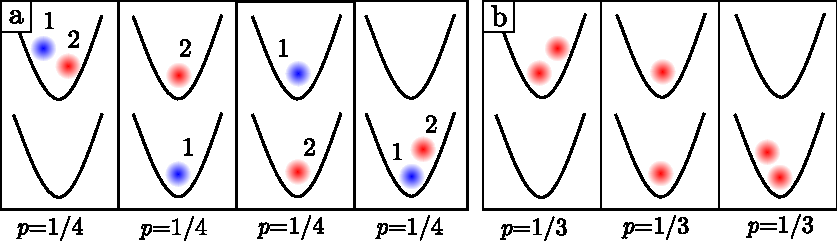
\includegraphics[width=\textwidth]{Fig/BEC_manip/stat_bose.pdf}
\caption{\textbf{a}: Répartition de deux particules discernables numérotées 1 et 2 sur deux niveaux d'énergie. Quatre configurations sont possibles. \textbf{b}: Répartition de deux particules indiscernables sur deux niveaux d'énergie. Dans le cas où ces particules peuvent se trouver dans le même état (bosons), trois configurations sont alors possibles.}
\label{fig:stat_bose}
\end{figure}

Considérons alors le cas simple de la répartition de deux particules sur deux niveaux d'énergie. Dans le cadre de la physique classique, il est possible d'attribuer un numéro à chaque particule, et il on peut placer chaque particule dans n'importe quel niveau d'énergie. Il existe alors quatre configurations que l'on supposera équiprobables, chacune de probabilité $p=1/4$ (voir figure \ref{fig:stat_bose}a). L'approche quantique, dans laquelle il n'est pas possible de discerner les particules, restreint le nombre de possibilités à trois et donc la probabilité de chacune des configurations est alors de $p=1/3$ (voir figure \ref{fig:stat_bose}b). Calculons maintenant la probabilité que deux particules soient dans le même état. En physique classique, cette probabilité est de $p=2/4=1/2$, tandis qu'en mécanique quantique, celle-ci est de $p=2/3$. On s'attend alors à ce que l'indiscernabilité des particules en mécanique quantique modifie la statistique de Boltzmann en favorisant l'agrégation de particules dans le même état \footnote{Ce raisonnement est valable pour des particules bosoniques, qui peuvent se retrouver dans le même état quantique. Pour des particules fermioniques, qui ne peuvent pas se retrouver dans le même état quantique, les statistiques en sont donc profondément changées. En guise d'illustration, la seule configuration possible de la figure \ref{fig:stat_bose}b pour des fermions est la seconde configuration.}.

\paragraph*{Condensation de Bose-Einstein}
Considérons alors le cas d'un gaz de $N$ bosons identiques dans un piège harmonique:
\begin{equation}
V(x,y,z)=\frac{1}{2}m \omega_x^2 x^2 + \frac{1}{2}m \omega_y^2 y^2 + \frac{1}{2}m \omega_z^2 z^2
\label{eq:piege_harmonique}
\end{equation}
où $m$ correspond à la masse des particules, et les $\omega_i$ correspondent aux fréquences de piégeage dans chaque direction de l'espace. Les énergies $E_{\mathbf{n}}$ sont donc celles des états liés
\begin{equation}
E_{\mathbf{n}}=\left(n_x+\frac{1}{2}\right) \hb \omega_x + \left(n_y+\frac{1}{2}\right) \hb \omega_y + \left(n_z+\frac{1}{2}\right) \hb \omega_z \quad \text{avec}\quad \mathbf{n}=\lbrace n_x,n_y,n_z\rbrace
\end{equation}

On peut alors montrer que le nombre moyen de particules est donné par la distribution de Bose-Einstein \footnote{Pour un gaz de $N$ fermions identiques, le nombre moyen de particules est donné par la distribution de Fermi-Dirac $ N_{\mathbf{n}}=\frac{g_{\mathbf{n}}}{\exp{\left( (E_{\mathbf{n}}-\mu)/k_{\mathrm{B}}T\right)}+1}$.}:\citep{diu1989elements}
\begin{equation}
N_{\mathbf{n}}=\frac{g_{\mathbf{n}}}{\exp{\left( (E_{\mathbf{n}}-\mu)/k_{\mathrm{B}}T \right)}-1}
\end{equation}
Une condition de validité de cette équation est que le potentiel chimique $\mu$ soit plus petit que l'énergie $E_{\mathbf{0}}$ du niveau de plus basse énergie, appelé niveau fondamental. Autrement, le nombre moyen de particules du niveau fondamental serait négatif (et cela impliquerait que la totalité du réservoir de particules vienne se déverser dans le niveau fondamental). Il est donc nécessaire que $\mu < E_0$. Une conséquence remarquable cette condition est que la population totale des états excités est bornée par:
\begin{equation}
N_e(\mu,T)=\sum_{\mathbf{n}\neq\mathbf{0}} N_{\mathbf{n}} \leq \sum_{\mathbf{n} \neq \mathbf{0}} \frac{g_{\mathbf{n}}}{\exp{\left( (E_{\mathbf{n}}-E_{\mathbf{0}})/k_{\mathrm{B}}T \right)}-1}
\end{equation}
Ainsi, chaque particule supplémentaire peuplera forcément l'état fondamental. On a donc ici le moyen d'accumuler un grand nombre de particules dans le même état quantique. La condensation de Bose-Einstein correspond, par définition, à cette accumulation d'un nombre macroscopique de particules dans l'état fondamental. Toutes ces particules peuplant cet état partagent alors le même état quantique. Afin d'atteindre un tel régime, il est nécessaire que les paquets d'onde des particules individuelles se recouvrent, c'est à dire que l'extension typique d'un paquet d'onde soit plus grande que la distance moyenne entre particules. L'extension typique de la fonction d'onde d'une particule peut être estimée à l'aide du principe d'incertitude de Heisenberg: $\Delta x \sim \hb / \Delta p$ avec $\Delta p \sim h/\lambda_{\mathrm{dB}}$. La grandeur $\lambda_{\mathrm{dB}}$ est homogène à une longueur et s'appelle la longueur d'onde thermique de de Broglie. Elle correspond à la taille typique d'un paquet d'onde quantique dont la largeur de la distribution en impulsion est donnée par la température. Celle-ci est donnée par \citep{diu1989elements}
\begin{equation}
\lambda_{\mathrm{dB}}=\sqrt{\frac{2\pi \hb^2}{m k_{\mathrm{B}}T}}
\end{equation}
avec m la masse de la particule, un atome de ${}^{87}$Rb dans le cas de notre expérience. La distance inter-particules dans un piège est estimée à partir de la densité de particules $d \sim n^{-1/3}$. On peut alors formuler le critère phénoménologique suivant:
\begin{equation}
n \lambda_{dB}^3 \gtrsim 1
\label{eq:critere_condensation}
\end{equation}
La quantité $n \lambda_{\mathrm{dB}}^3$ est appelée \emph{densité dans l'espace des phases}. Tout l'enjeu des expériences d'atomes ultrafroids est d'arriver à augmenter la densité dans l'espace des phases afin de franchir le seuil donné par l'équation \ref{eq:critere_condensation}. Cette condition peut se réécrire en terme de \emph{température critique}:
\begin{equation}
T_{\mathrm{C}}\sim \frac{\hb \overline{\omega}}{k_{\mathrm{B}}}N^{1/3}
\label{eq:temperature_critique}
\end{equation}
où $\overline{\omega}=(\omega_x \omega_y \omega_z)^{1/3}$ est la fréquence moyenne du piège. Cette température critique est de l'ordre de quelques centaines de nano-kelvin pour les expériences typiques d'atomes ultra-froids.


\subsection{Propriétés d'un condensat de Bose-Einstein}
En dessous de la température critique \ref{eq:temperature_critique}, les atomes s'accumulent dans l'état fondamental du piège. Il en résulte une forte augmentation de la densité, si bien qu'on ne peut plus négliger les interactions entre particules. Dans le cas d'un gaz suffisamment dilué, ce que l'on considèrera dans la suite, les interactions entre atomes peuvent être traitées comme des collisions à basse énergie, c'est à dire des collisions uniquement dans l'onde \emph{s}. Le potentiel d'interaction est alors celui de contact, donné par $U(\mathbf{r}_1-\mathbf{r}_2)=g\delta(\mathbf{r}_1-\mathbf{r}_2)$. Le paramètre $g$, qui caractérise la force des interactions, est donné par $g=\frac{4 \pi \hb^2}{m}a_{\mathrm{s}}$, avec $a_{\mathrm{s}}$ la longueur de diffusion, et ne dépend que de ce paramètre. Ce régime dilué est atteint lorsque $na_{\mathrm{s}}^3\ll 1$\footnote{Dans ce régime, la distance inter-atomique est plus grande que la portée des interactions. Ainsi, les atomes ne voient pas le détail du potentiel d'interaction avec leur voisin, et donc il est possible d'approximer ce potentiel par un potentiel de contact.}. Pour le ${}^{87}$Rb, cette longueur de diffusion vaut 100$a_{\mathrm{0}}>0$, avec $a_{\mathrm{0}}$ le rayon de Bohr. La longueur de diffusion étant positive, les interactions sont donc répulsives pour notre atome.

On peut écrire l'équation de Schrödinger pour l'état fondamental en tenant compte de ce terme d'interaction entre particules. La description en champ moyen du condensat est alors donnée par l'équation de Gross-Pitaevskii (aussi connue sous le nom d'\emph{équation de Schrödinger non-linéaire}):
\begin{equation}
i\hb \frac{\partial}{\partial t} \psi(\mathbf{r},t)=\left[-\frac{\hb^2}{2m}\Delta +V(\mathrm{r})+g\left| \psi(\mathbf{r},t) \right|^2 \right] \psi(\mathbf{r},t)
\label{eq:gross_pitaevskii}
\end{equation}
où $\psi(\mathbf{r},t)$ est la fonction d'onde macroscopique du condensat. La densité d'atomes est donnée par $n(\mathbf{r})= \left| \psi(\mathbf{r}) \right|^2$. Ainsi, la fonction d'onde du condensat $\psi(\mathbf{r},t)$ est normalisée pour donner le nombre de particules dans le condensat:
\begin{equation}
\int{\mathrm{d}\mathbf{r} \: \left| \psi(\mathbf{r},t) \right|^2}=N_{\mathbf{0}}
\end{equation}
Dans le régime stationnaire, on peut écrire $\psi(\mathbf{r},t)=\psi_0(\mathbf{r}) e^{i\mu t/\hb}$ avec $\mu$ le potentiel chimique du condensat, et l'injecter dans l'équation \ref{eq:gross_pitaevskii}. On obtient l'équation de Gross-Pitaevskii stationnaire:
\begin{equation}
\left[ -\frac{\hb^2}{2m}\Delta + V(\mathbf{r}) + g\left|\phi_0(\mathbf{r})\right|^2 \right] \phi_0((\mathbf{r}) = \mu \phi_0(\mathbf{r})
\end{equation}
Le premier terme de gauche décrit l'énergie cinétique, le second le terme d'énergie potentielle provenant du piège, et le dernier décrit l'énergie d'interaction entre particules, proportionnelle à la densité locale $n(\mathbf{r})=\left| \psi(\mathbf{r})\right|^2=\left| \phi_0(\mathbf{r}) \right|^2$. La somme de ces énergies donne le potentiel chimique $\mu$, qui correspond à l'énergie qu'il faut fournir pour rajouter une particule supplémentaire au système de $N$ particules.

\paragraph*{Régime de Thomas-Fermi}
Considérons le cas d'un condensat comportant un grand nombre de particules $N_0$. L'énergie cinétique totale du condensat varie avec $N_0$ de manière linéaire: $\mean{E_{\mathrm{k}}}\propto N_0$. L'énergie totale d'interaction varie quant à elle en $E_{\mathrm{int}}\propto N_0^2$. Pour un nombre suffisamment grand de particules, il devient possible de négliger le terme d'énergie cinétique dans l'équation de Gross-Pitaevskii stationnaire: il s'agit du régime de Thomas-Fermi.
Dans ce cas, le profil de densité s'écrit
\begin{equation}
n(\mathbf{r})=\left\{
					\begin{array}{ll}
						(\mu-V(\mathbf{r}))/g &\quad \text{lorsque} \quad \mu>V(\mathbf{r})\\
						0 &\quad \text{sinon}
					\end{array} 
				\right.
\end{equation}
et en considérant le piège harmonique de l'équation \ref{eq:piege_harmonique},
\begin{equation}
n(\mathbf{r})=\left\{
					\begin{array}{ll}
						\mu/g-\sum_{i=x,y,z}\frac{m\omega_i^2}{2g}r_i^2 &\quad \text{lorsque} \quad \mu>V(\mathbf{r})\\
						0 &\quad \text{sinon}
					\end{array} 
				\right.
\end{equation}
Le profil de densité est donc une parabole inversée de rayons
\begin{equation}
r_{\mathrm{TF},i}=\sqrt{\frac{2\mu}{m\omega_i^2}}
\end{equation}
Ces rayons ont été déterminés par la condition $n(\mathbf{r})=0$. Il est intéressant de noter que le potentiel effectif vu par une particule $V_{\mathrm{eff}}(\mathbf{r})=V(\mathbf{r})+gn(\mathbf{r})$ est constant sur l'ensemble du condensat:
\begin{equation}
V_{\mathrm{eff}}(\mathbf{r})= \left\{
									\begin{array}{ll}
										\mu &\quad \text{lorsque} \quad \mu>V(\mathbf{r})\\
										V(\mathbf{r}) &\quad \text{sinon}
									\end{array}
							\right.
\end{equation}
Enfin, il est possible d'obtenir une expression pour le potentiel chimique \citep{pethick2008bose}: 
\begin{equation}
\mu=\frac{1}{2} \left( 15a N_{\mathbf{0}} \hb^2 \overline{\omega}^3 \right) ^{2/5} m^{1/5}
\end{equation}
et vaut environ $\mu/h\approx40$Hz pour notre expérience.

En réalité, l'approximation de Thomas-Fermi décrit bien les zones à l'intérieur des condensats, cependant, il existe une petite région sur les bords du condensat où la densité est faible, et donc l'énergie cinétique ne peut plus être négligée devant l'énergie d'interaction. Cette échelle de longueur s'appelle la longueur de cicatrisation, donnée par 
\begin{equation}
\xi=\sqrt{\frac{\hb^2}{n_{\mathbf{0}} mg}}
\end{equation}
avec $n_{\mathbf{0}}$ la ensité moyenne du condensat. $\xi$ représente donc la longueur sur laquelle le potentiel chimique n'écrante pas le potentiel externe.


\section{Processus d'interaction lumière-matière} 
\subsection{Potentiel dipolaire}
\subsection{Force de pression de radiation}
\subsection{Potentiel magnétique}
\subsection{Couplage radio-fréquence} 

\section{Description d'un cycle expérimental}
\subsection{Première chambre}
\subsection{Chambre de science}
\subsection{Imagerie}




\begin{comment}
%Chapter 3: A cognitive experiment to study confidence
%------------------------

%3.1 : Experimental procedure
%- In humans
%- In animals


%3.2 : Our procedure


%% Intro à retravailler

Confidence judgments in one's decision are considered a central example of metacognition. How can we access to the subjective sense of confidence of someone else ? In this chapter, I will review to different behavioral measures to obtain this sense of confidence in humans and in animals. In a second part, I will present the experiment I performed, in collaboration with Jean-R\'emy Martin and J\'er\^ome Sackur at ENS, during my PhD. 


\section{How to measure confidence experimentally ?}

%% plus  de refs si le temps

%% exemple des histogrammes et des performances etc ....
%% une partie sur les inconvenients d'une telle méthode
% https://link.springer.com/article/10.3758/s13423-018-1553-3

\subsection{In Humans} %% titre à changer

\paragraph*{Explicit reports of confidence}
Reports of confidence in humans can be made explicit through verbal communications for example.Thus, the most straightforward paradigm to measure confidence is to ask the subjects to assign a numerical rating in how sure they are in their answer at each trial. %% REFS
They provide a subjective probability on the correctness of their response as a confidence judgment.
One important aspect of such reports is that performance accuracy and response times are well-correlated with self-confidence reports. %ù REFS
This phenomena occurs for a variety of tasks such as general knowledge tests~\citep{perfect1993accuracy}, perceptual decisions~\citep{fleming2010relating} and reasoning tasks~\citep{stankov2000complexity}.
%% Figure suivante faite grâce à la base de donnée confidence database Adler & ma 2018 exp 2
In Figure ???, I represent an example of such relation between these behavioral variables. The experiment consisted in a categorization task (with Gabor patches) followed by a confidence judgment on a four-points scale. %% REF Adlmer
The data are publicly shared through the {\em confidence databse} project. %% REFS
The most striking effect that appears from having access to direct reports of confidence is the {\em under/over-confidence}~\citep{lichtenstein1977those}. %% A lire plus en détails TODO TODO TODO ++++
These deviations occur systematically with overconfidence when the decisions are difficult and underconfidence for easy decisions~\citep{Kepecs_A_2012}. 
However, it is worth noting that these biases in confidence vary greatly with the type of judgments that are asked, and across participants~\citep{klayman1999overconfidence}. %% Figure overconfidence à faire en exemple

%% remarque sur version cntinue, discrète ou combien d'échelon



%% un mot sur les autres méthodes
\paragraph*{Other measures of confidence}

%\paragraph*{Post-decision wagering} for exemple

%% lire les autres articles pour bien comprendre les critiques/remarques
%% lesm oyens de mesures sont très variés (article Pascal M.)

%% formulatio à revoir
\subsection{In animals}
For animals, one can not simply ask them to explicitly report their confidence. Therefore, more sophisticated tasks have been employed to elicit a report of confidence in animals.

\paragraph*{Uncertain option task} %%%REFS ??? et article shadlen ?
One of the most common task used for this purpose is the {\em uncertain option} task. It extends the classical two-choices paradigm that has been mentioned in this thesis. In addition to the two available responses, the animal is offered a third choice, that will correspond to a small but certain reward. This framework has been used in many species such as monkeys, dolphin and rats. %% REFS 
Interestingly, when compared to human performances on this type of task, dolphin and monkeys showed qualitative similar strategies and response distributions. However, one can address the following criticism to this kind of task: there is the possibility that this task is considered as a three-choices task by the animal. The animal could be learning the association between the uncertain reward and a difficult task. 


\paragraph*{Opt-out task}
% expliquer marche pas avec rat (sauf exception) et donc les exp. suivantes
% fig inkscape opt-out task
To address this problematic,~\cite{hampton2001rhesus} developed a modified version of the uncertain option task. It consists in a memory task in which monkeys perform a delayed-maching-to-sample task. At the end of delay, monkeys were presented with the option of declining or accepting the discrimination test. Moreover,~\cite{hampton2001rhesus} imposed that on some trials the monkeys have no choice but to make the discrimination test. This is to ensure that the monkey is not learning to associate longer delay with {\em opt-out option}. They found that, the performances of the monkeys on freely chosen trials are greater than the ones in forced choice trials. 
This opt-out task as been used in macaque monkeys too~\citep{kiani2009representation,komura2013responses}, but in binary categorization of visual motion task. They found that the frequency of choosing the opt-out option increased with stimulus difficulty, as well as greater performances on freely chosen trials. Interestingly, this task has been tested in pigeons and rats %% REFS
but they don't find a change in performances between forced-choices and free-choices. These results raised the question or whether these animals could perform confidence judgments or not.



\paragraph*{Decision restart and leaving decision tasks}
%% un mot sur les problematiques de cette tache ?


In order to address the criticisms of two previous paradigms, such as the fact that, for these paradigms, either a confidence report either a decision report is collected at each trial,~\cite{Kepecs_A_2012} proposed a new paradigm in rodents. %% Figure %ù TODO phrase un peu longue ???
The rats were trained to perform a 2AFC olfactory discrimination task. Depending on the dominant part of the odour mixture, the rats need to choice the left or the right. A variable delay was imposed after a correct trial and the animal could restart the trial at will (Figure ???). There was no feedback on error trials which allow to measure the rats confidence in these trials. For some of the correct trials, the reward was omitted which allow to measure confidence for correct trials too. It has been found that the waiting time increased with respect to odour contrast for correct trials, but decreased for error trials. Moreover, accuracy was an increasing function of the waiting time. This suggests that the waiting time of each trial consists in a robust proxy for confidence.


\begin{figure}[h!]
	\centering
	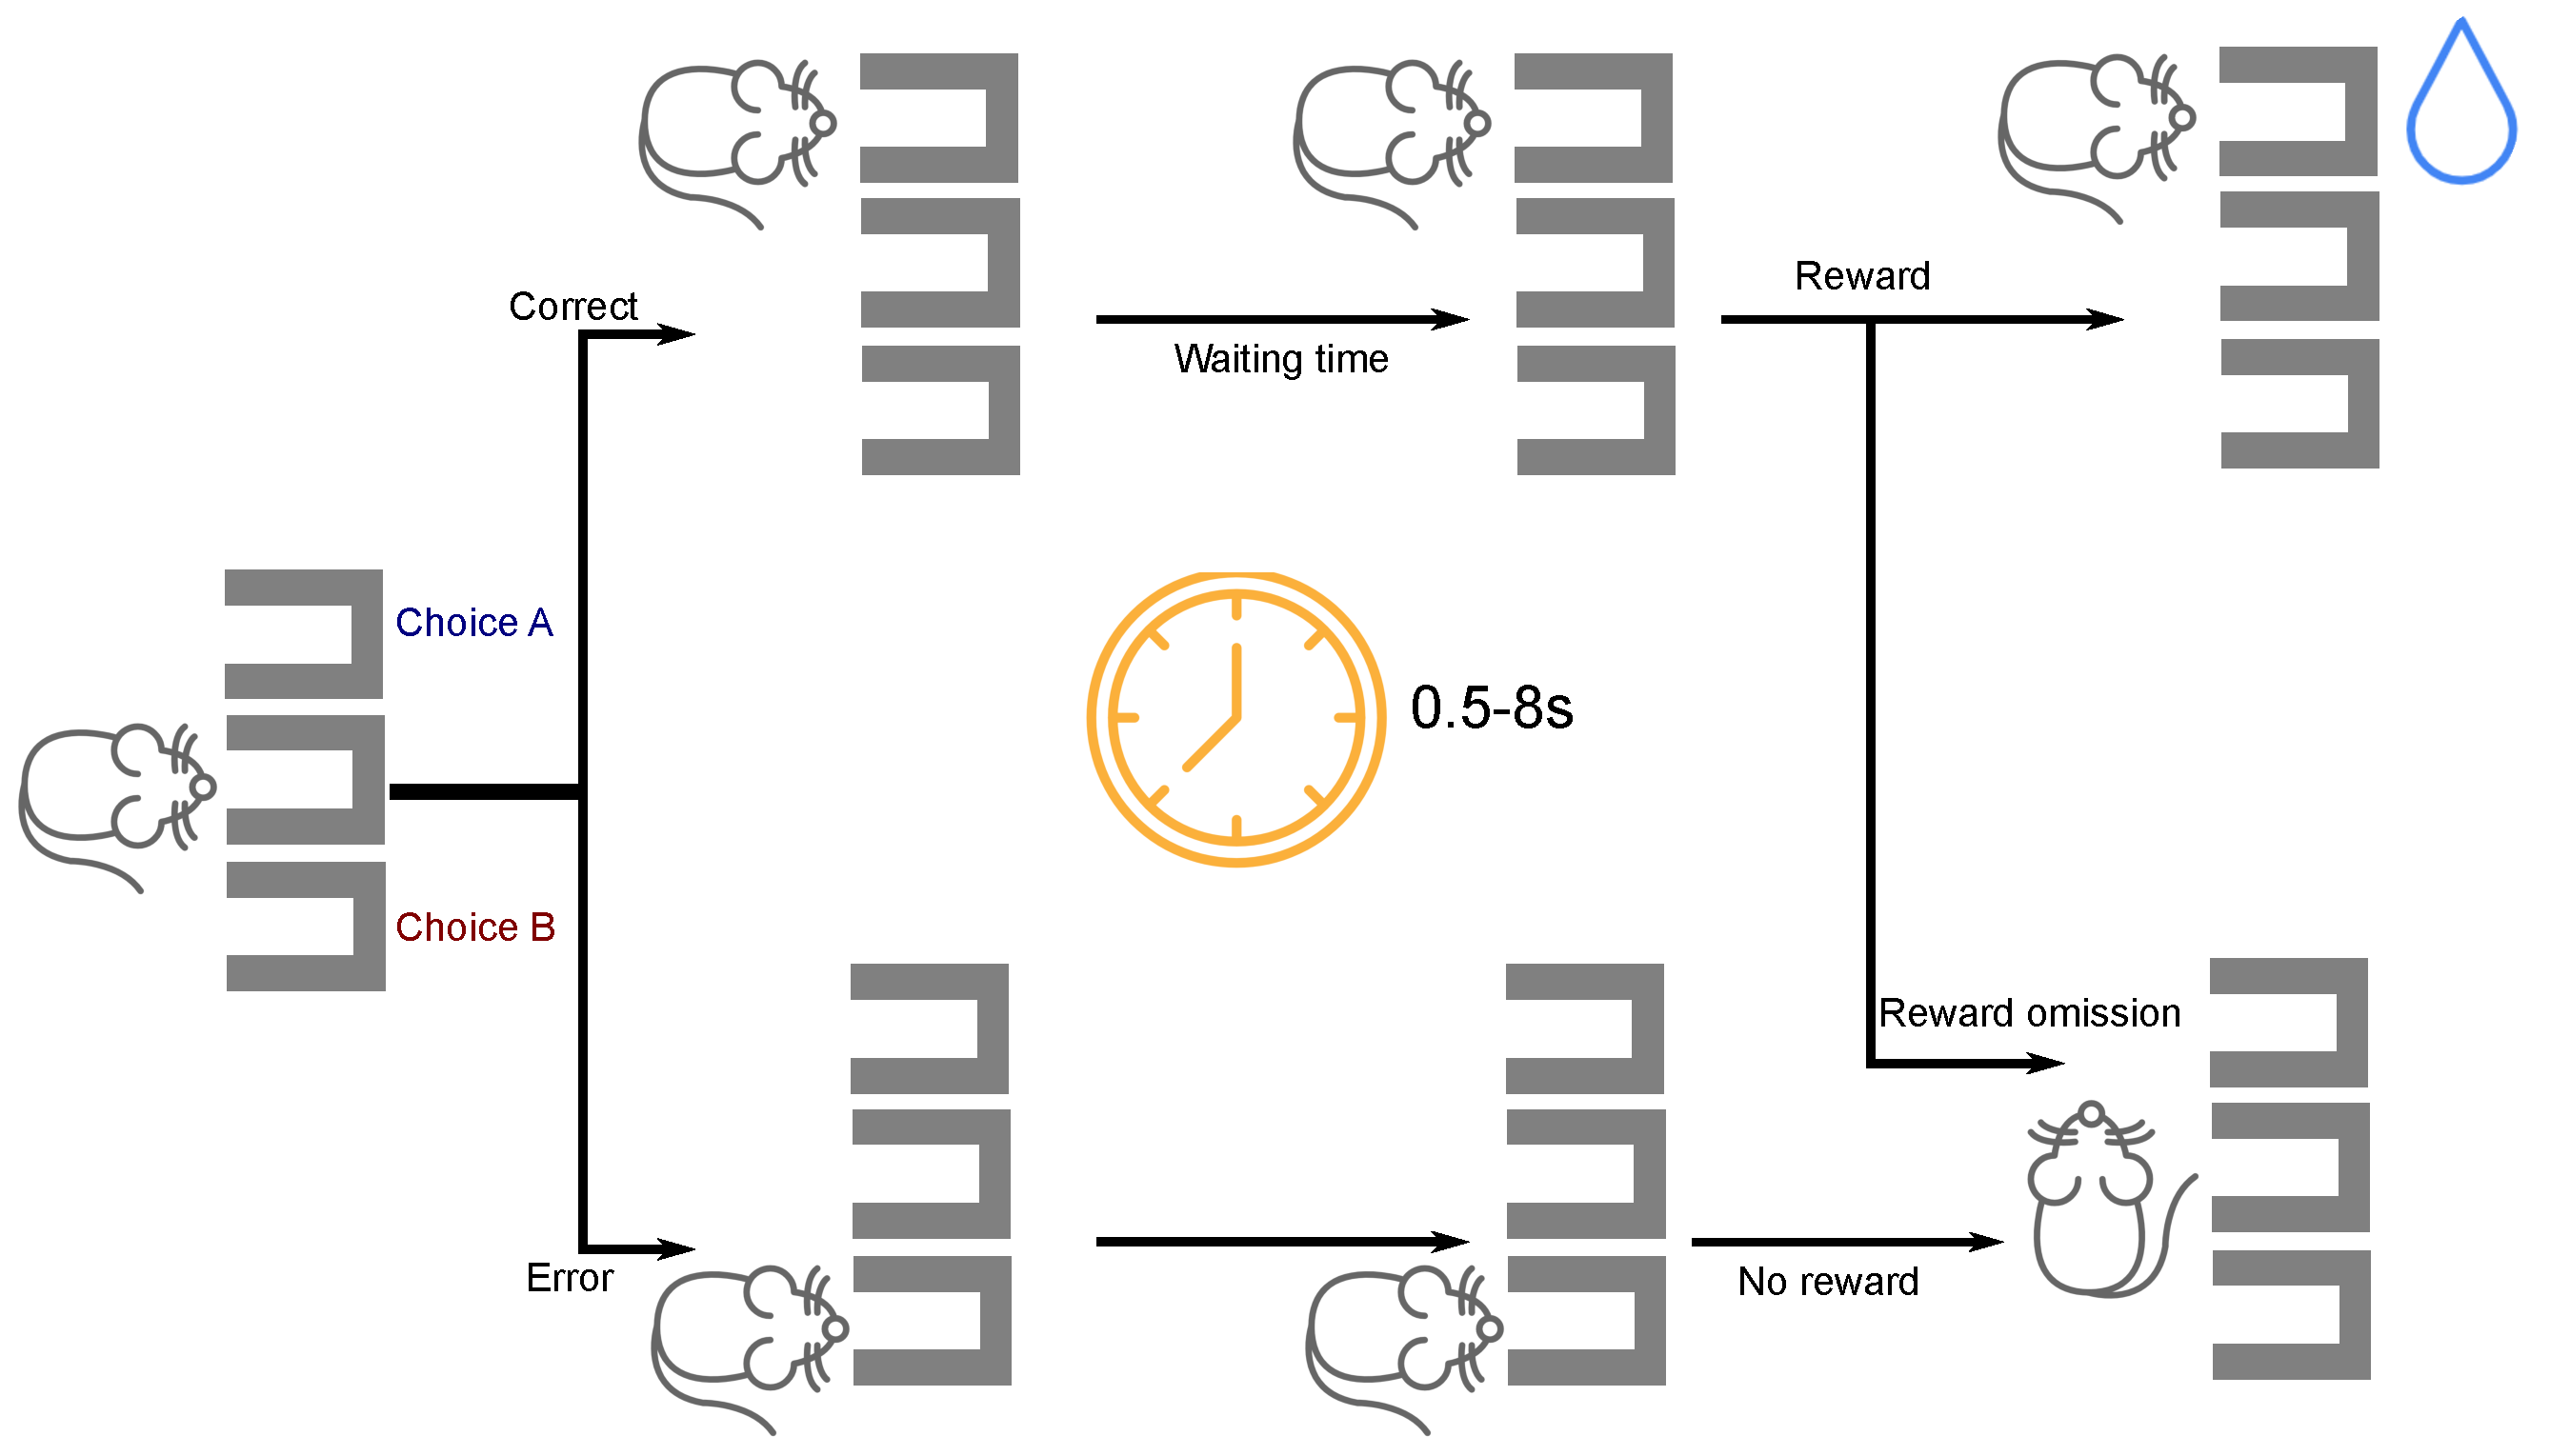
\includegraphics[width=0.7\linewidth]{Fig/Chapter3/confidence-souris.eps}
	\caption{{\bf }
	}
	\label{fig:fig6}
\end{figure}

%% conclusion de la section ????


\section{My experiment}

In this section I will describe the cognitive experiment that I have performed to study decision-making and confidence in humans. Previously to the design of this experiment, I briefly analyzed the results of an experiment of Jean-R\'emy Martin and J\'er\^ome Saclur within the framework of attractor neural network. The preliminary results led to the design of an experiment whose goal was to study the impact of confidence on decision-making and various sequential effects.


\subsection{Experimental set-up}
The experiment was performed at the Laboratoire de Psychologie cognitive et de Psycholinguistique’s database (LSCP, DEC, ENS-EHESS-CNRS, PSL, Paris, France). The experiment followed the ethics requirements of the Declaration of Helsinki (2008) and has been approved by the local Ethics Committee. It consists in a direction categorization task, where participants classify Gabor patches as clockwise or anti-clockwise. In some of the trials, the decision was followed by an auditory feedback or a confidence evaluation.

%% photo des salles de manip
The stimuli were generated using Matlab along with the Psychophysics toolbox. %% PERFS
The ywere displayed on a monitor at $57.3$~cm of the particpants head. The participants performed the experiment
in a quiet and darkened experimental room. Their heads were stabilized thanks to a chin-rest. %% Figure ????
The instructions to the participants (translated from french) were the following (the emphazised sentences correspond to additional information not provided to the participants):
\begin{itemize}
	\item In each trial, you will see very briefly ({\em $200$~ms}) a black dot at the center of the screen that you will need to look at (Figure~\ref{fig:consignes1}.A). Just after the dot dissappears ({\em ???~ms}), you will see a circular grating at the center of the screen like the one in Figure~\ref{fig:consignes1}.B. {\em The parameters of the circular grating are diameter = $4^{\circ}$, Tukey window, 2 cycles per degree, Michelson contrast = $89\%$, duration = $100$~ms, phase randomly selected at each trial.}
	
	\begin{figure}[h!]
		\begin{subfigure}{.5\textwidth}
			\centering
			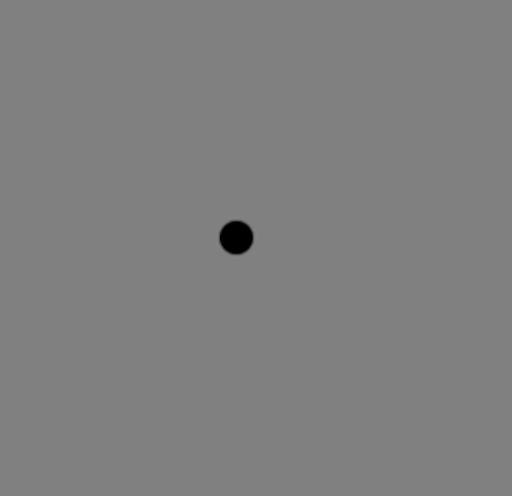
\includegraphics[width=.8\linewidth]{fig/Chapter3/fixation-dot.png}
			\caption{Fixation dot}
		\end{subfigure}%
		\begin{subfigure}{.5\textwidth}
			\centering
			
\includegraphics[width=.8\linewidth]{fig/Chapter3/0-grating.png}
			\caption{Example of the circular grating.}
		\end{subfigure}
		\caption{}
		\label{fig:consignes1}
	\end{figure}
	
	
	
	\item In each trial you will need to indicate if the grating was oriented clockwise or anti-clockwise (Figure~\ref{fig:consignes2}).
	\item As soon as the disk dissappears, if you think it was anti-clockwise oriented you will press the left directionnal arrow. If it was clockwise oriented you will press the right directionnal arrow.
	
		\begin{figure}[h!]
		\begin{subfigure}{.5\textwidth}
			\centering
			
\includegraphics[width=.8\linewidth]{fig/Chapter3/left-grating.png}
			\caption{Anti-clockwise circular grating.}
		\end{subfigure}%
		\begin{subfigure}{.5\textwidth}
			\centering
			
\includegraphics[width=.8\linewidth]{fig/Chapter3/right-grating.png}
			\caption{Clockwise circular grating.}
		\end{subfigure}
		\caption{}
		\label{fig:consignes2}
	\end{figure}
	
	
	\item In the case where you don't know at all which direction it was you will still press one of the two keys by following your intuition. When this happens, do not press always the same key.
	\item You need to answer fast but not at the expense of accuracy. After $1.5$ second, you will see a message at the screen "Please, answer". The ideal situation is to answer before this text appears at the screen.
	\item You will have $3$ bocks of trials:
	\begin{itemize}
		\item In the first block, once you have answered to a trial, the software will automatically run the next trial.
		\item  In a second block, you will receive a feedback on your answer at each trial. If the answer was correct, you will hear a pitched tone. If your answer was wrong you will hear a deep tone.
		\item In a third block, you will need to evaluate your confidence level in your answer using the scale that will appear on the screen (Figure ??). You will move the black slider towards right or left using the left and right stickers on the keyboard (q and e keys). The scale is composed of $10$ levels. The case at the left corresponds to the "Pure guessing" case. You choose randomly the orientation of the grating. At the right you have the "Certain to be sure" case. You are absolutely certain to be right, there is no possible doubt. Between these two cases, you have access to intermediate levels of confidence. The choice of the confidence level is performed using the space bar.
			
			
				\begin{figure}[h!]
					\centering
					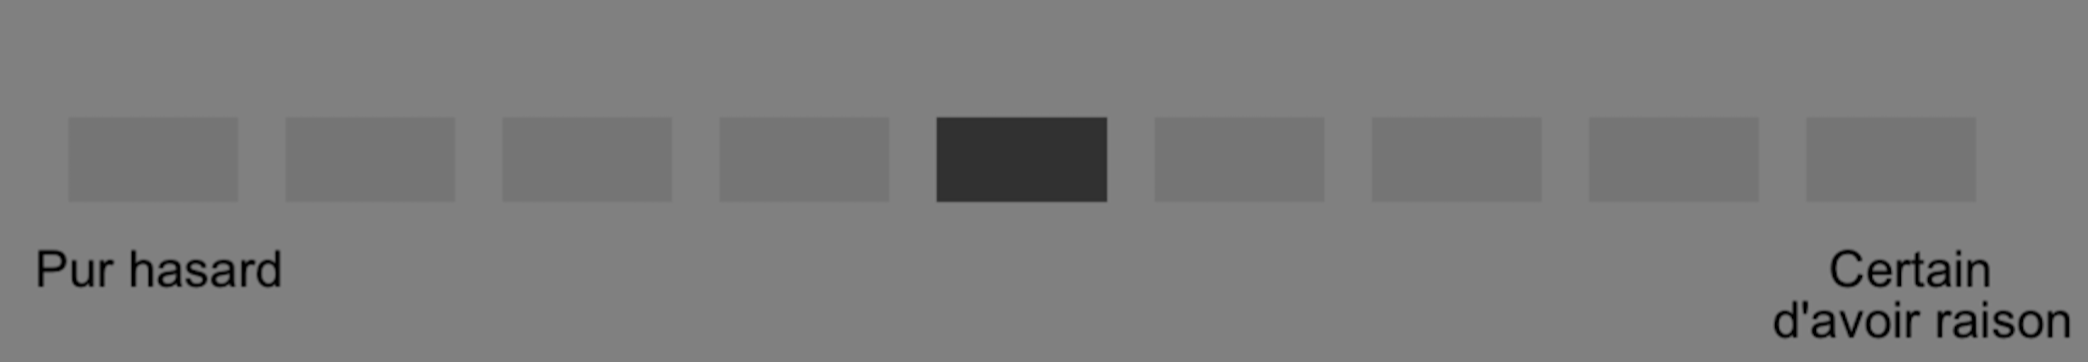
\includegraphics[width=.8\linewidth]{fig/Chapter3/scale-confidence.png}
					\caption{Confidence-scale.}
					\label{fig:consignes3}
			\end{figure}
			
			
			
	\end{itemize}
\item Be aware that, in the confidence block, the black slider will appear randomly on the scale. Don't be biased by the initial position of the cursor and move it o the level that reflets your level of confidence.
\item During the confidence block, in the case you wanted to choose the right arrows but you chose the left one (or inversely), don't answer to the confidence scale. Just press the keyboard key with a red sticker on it, it will go to the next trial.
\item The software will choose the order of the block and you will know at the beginning of each block which one it is. Before the main experiment starts, you will have a small training.
\end{itemize}

Nine participants (7 Females, Mean Age = 27.3, SD = 5.14) have been recruited from the Laboratoire de Psychologie cognitive et de Psycholinguistique’s database (LSCP, DEC, ENS-EHESS-CNRS, PSL, Paris, France).
Every subject had normal or corrected-to-normal vision. The participants performed three sessions on three distinct days in the same week for a total duration of about 2h15. Three participants were excluded. Two of the excluded participants did not complete correctly the experiment and one exhibited substantially asymmetric performance
($98\%$ of correct responses for an angle of 0.2\textdegree, but $18\%$ at -0.2\textdegree degree). As a result, we analyzed data from 6 participants. We obtained written informed consent from every participant who received a compensation of 15 euros for their participation. 
Participants performed three sessions on three distinct days. Each session ($45$~min) consisted in three runs, each run being composed of one exemplar of each of the three type of block, in a random order.




\subsection{Experimental procedure}

The experimental procedure is shown in Figure ??. The waiting time between each trial was deliberatly chosen to be low, and similar between blocks, to study the sequential effects.



\paragraph*{Pure block} 
In this block, participants waited $300$~ms after each decision, before the black fixation point appears. The stimulus appeared $200$~ms after this fixation point. The eight possible orientations for the circular grating were [-1.6\textdegree, -0.8\textdegree, -0.5\textdegree, -0.2\textdegree , 0.2\textdegree , 0.5\textdegree , 0.8\textdegree , 1.6\textdegree  ] and a stimulus was chosen randomly among them with the following weights: [0.05, 0.1, 0.15, 0.2, 0.2, 0.15, 0.1, 0.05]. 

\paragraph*{Feedback block}
In this block, $200$~ms after the decision, the participants received an auditory feedback (during $200$~ms) about the correctness of the decision they just made. The black fixation dot appeared $100$~ms after this feedback and a new trial began. The orientations of the circular gratings were chosen randomly from [-1.6\textdegree, -0.8\textdegree,  -0.2\textdegree , 0.2\textdegree ,  0.8\textdegree , 1.6\textdegree  ] with the following weights [ 0.12, 0.18, 0.2, 0.2, 0.18, 0.12 ].


\paragraph*{Confidence block} In the confidence block, participants had to evaluate the confidence on the orientation task $200$~ms after the decision. After the choice of confidence, the participants had to wait $300$~ms before the black fixation dot appears. After the fixation dot the stimulus appeared $200$~ms later. The orientations of the circular gratings were the same as in the feedback block. 

%%% différents résultats des performances etc ....
%% testi nfluence block confiance

I will present different results from this experiment, without the framework of attractor network that will be discussed in the next chapter of this manuscript. 



\end{comment}


